\documentclass[10pt]{article}
\usepackage[a4paper,margin=18mm]{geometry}
\usepackage[T1]{fontenc}\usepackage{lmodern}
\usepackage{amsmath,amssymb,booktabs,array,enumitem}
\usepackage{tikz}\usetikzlibrary{shapes.gates.logic.US,positioning,arrows.meta}
\usepackage[hidelinks]{hyperref}
\setlength{\parindent}{0pt}\setlength{\parskip}{4pt}\setlength{\emergencystretch}{2em}
\newcommand{\mos}[4]{\begin{scope}[shift={(#1,#2)}]
\draw(0,.24)--(0,-.24);\draw(0,.2)--(.25,.2)--(.25,.5);\draw(0,-.2)--(.25,-.2)--(.25,-.5);
\draw(-.16,.23)--(-.16,-.23);
\ifnum#4=1\draw(-.26,0)circle(.06);\draw(-.75,0)--(-.32,0);\else\draw(-.75,0)--(-.16,0);\fi
\node[anchor=east,font=\scriptsize]at(-.76,0){$#3$};\end{scope}}
\newcommand{\gnd}[2]{\draw(#1,#2)--(#1,{#2-.12});\draw({#1-.17},{#2-.12})--({#1+.17},{#2-.12});\draw({#1-.11},{#2-.2})--({#1+.11},{#2-.2});}
\newcommand{\rail}[3]{\draw(#1,#2)--(#1,{#2+.14});\node[above,font=\scriptsize]at(#1,{#2+.14}){$#3$};}
\begin{document}
\begin{center}\large\textbf{EE3032 Introduction to VLSI -- Midterm}\\\normalsize Fall 2023: available latter questions\end{center}
\textbf{Source coverage.} Only original page 2-2 is available. Questions 5--7 are complete (35 printed points). Questions 1--3 and the opening of Question 4 are unavailable; they are not reconstructed from student answers.

\textbf{Question 4 continuation (incomplete; opening and parameters missing).}\\
\emph{[The source begins mid-sentence:]} ``voltage of the output $V_{out}$ is $1.2\,\mathrm V$ and an input stimulus $(0\to1.2\,\mathrm V)$ as shown in Fig. 3(b) is applied, how much voltage of the input stimulus $(V_{in})$ at $x$ is? (4 points) Identify the operation region of the transistors N1, N2, and N3 from $t_1$ to $t_2$. (6 points)''
\begin{center}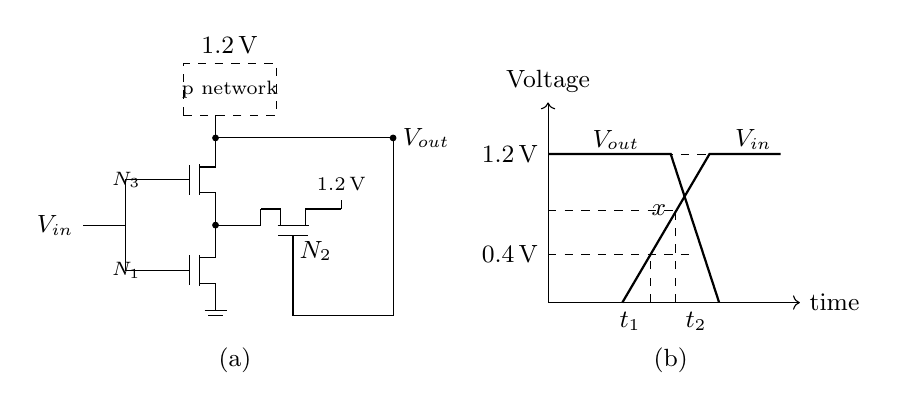
\begin{tikzpicture}[scale=.82,font=\small]
\draw[dashed](-.25,3.5)rectangle(1.2,4.3);\node[font=\scriptsize]at(.47,3.9){p network};\node[above]at(.47,4.3){$1.2\,\mathrm V$};
\draw(.25,3.5)--(.25,3.0);\mos{0}{2.5}{N_3}{0}\mos{0}{1.1}{N_1}{0}
\draw(.25,2)--(.25,1.6);\gnd{.25}{.6}
\draw(-.75,2.5)--(-1.15,2.5)--(-1.15,1.1)--(-.75,1.1);\draw(-1.15,1.8)--(-1.8,1.8)node[left]{$V_{in}$};
\draw(.25,3.15)--(3,3.15)node[right]{$V_{out}$};\fill(.25,3.15)circle(1.5pt);
\begin{scope}[shift={(1.45,1.8)},rotate=90]\mos{0}{0}{}{0}\end{scope}
\draw(.25,1.8)--(.95,1.8)--(.95,2.05);\fill(.25,1.8)circle(1.5pt);
\draw(1.95,2.05)--(2.2,2.05);\rail{2.2}{2.05}{1.2\,\mathrm V};\node at(1.8,1.4){$N_2$};
\draw(1.45,1.05)--(1.45,.4)--(3,.4)--(3,3.15);\fill(3,3.15)circle(1.5pt);
\begin{scope}[xshift=1.4cm]
\draw[->](4.0,.6)--(7.9,.6)node[right]{time};\draw[->](4,.6)--(4,3.7)node[above]{Voltage};
\draw[dashed](4,2.9)--(6.9,2.9);\node[left]at(4,2.9){$1.2\,\mathrm V$};
\draw[dashed](4,1.35)--(6.2,1.35);\node[left]at(4,1.35){$0.4\,\mathrm V$};
\draw[thick](4,2.9)--(5.9,2.9)--(6.65,.6);\node at(5.05,3.12){$V_{out}$};
\draw[thick](5.15,.6)--(6.5,2.9)--(7.6,2.9);\node at(7.18,3.13){$V_{in}$};
\draw[dashed](5.58,.6)--(5.58,1.35);\draw[dashed](5.98,.6)--(5.98,2.03);\node[below left]at(5.58,.6){$t_1$};\node[below right]at(5.98,.6){$t_2$};
\draw[dashed](4,2.03)--(5.98,2.03);\node[left]at(5.98,2.03){$x$};
\node at(5.9,-.3){(b)};\end{scope}\node at(.55,-.3){(a)};
\end{tikzpicture}\\Figure 3: (a) A CMOS logic gate. (b) Waveforms of $V_{in}$ and $V_{out}$.\end{center}\textbf{5. (10 points)} Fig. 4(a) shows a CMOS circuit. Assume that the sizes of NMOS and PMOS transistors in the logic gates are $W/L$ and $2W/L$, respectively. Also, $\mu_n=2\mu_p$. If the functional inputs of the circuits are
$(ABCD)=\{0011,0101,1101,1110\}$, explain the relationship of noise margins $NM_L$ and $NM_H$ (i.e., $NM_L>NM_H$, $NM_L<NM_H$, or $NM_L=NM_H$) of each gate.\begin{center}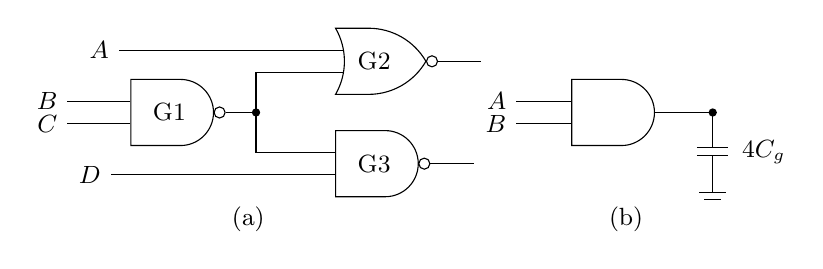
\begin{tikzpicture}[font=\small]
\node[nand gate US,draw,logic gate inputs=nn,logic gate input sep=.28cm](g1)at(0,0){G1};
\node[nor gate US,draw,logic gate inputs=nn,logic gate input sep=.28cm](g2)at(2.6,.65){G2};
\node[nand gate US,draw,logic gate inputs=nn,logic gate input sep=.28cm](g3)at(2.6,-.65){G3};
\draw(g1.input 1)--++(-.8,0)node[left]{$B$};\draw(g1.input 2)--++(-.8,0)node[left]{$C$};
\draw(g2.input 1)--++(-2.85,0)node[left]{$A$};\draw(g3.input 2)--++(-2.85,0)node[left]{$D$};
\draw(g1.output)--(1.1,0);\draw(1.1,0)|-(g2.input 2);\draw(1.1,0)|-(g3.input 1);\fill(1.1,0)circle(1.5pt);
\draw(g2.output)--++(.55,0);\draw(g3.output)--++(.55,0);\node at(1,-1.35){(a)};
\node[and gate US,draw,logic gate inputs=nn,logic gate input sep=.28cm](a)at(5.6,0){};
\draw(a.input 1)--++(-.7,0)node[left]{$A$};\draw(a.input 2)--++(-.7,0)node[left]{$B$};
\draw(a.output)--(6.9,0);\fill(6.9,0)circle(1.5pt);\draw(6.9,0)--(6.9,-.45);
\draw(6.7,-.45)--(7.1,-.45);\draw(6.7,-.55)--(7.1,-.55);\gnd{6.9}{-.9};\draw(6.9,-.55)--(6.9,-.9);\node[right]at(7.15,-.5){$4C_g$};\node at(5.8,-1.35){(b)};
\end{tikzpicture}\\Figure 4: CMOS circuits.\end{center}\newpage
\begin{center}\large\textbf{Complete questions (continued)}\end{center}
\textbf{6. (10 points)} For a given technology, the turn-on resistance of a $W/L$ NMOS is $R$ and $\mu_n=2\mu_p$. Also, the gate capacitance of a $W/L$ NMOS or PMOS transistor is $C_g$. Fig. 4(b) shows a two-input AND gate drives a $4C_g$ capacitive load. Design the AND gate such that the worst-case delay of the AND gate is smaller than $8RC_g$, where the delay is estimated by using simple RC model and the parasitic capacitance can be ignored. Draw the transistor-level schematic diagram and label the size of each transistor in terms of $W/L$.\par\vspace{17mm}\par\textbf{7. (15 points)} Realize the following Boolean functions using CMOS logic:
\begin{enumerate}[label=(\alph*),leftmargin=8mm]
\item $F=X(Y+Z)+XW$. (5 points)
\item $F=\overline{X(Y+Z)}$. (5 points)
\item $F=XY+YZ$. (5 points)
\end{enumerate}\vfill
\textit{Retained complete-question total: 35 points. The visible Q4 continuation carries 4+6 points, but its missing premise prevents a complete answer. Original Figure 2 belongs to an absent earlier question and is preserved only in the source PDF.}
\end{document}
